\section{Introduction}

The Internet has enabled billions of people around the world to connect, communicate, and cooperate. However, even the most widely spoken language, Mandarin, is only spoken by 12\% of the world population. 
Other official languages of the United Nations, like English and French, are only spoken by 4.8\% and 1.0\% of the world, respectively \cite{I1}. 
Even if we include non-native speakers who are able to communicate in that language, they still only represent 12\% and 3\% of the world, respectively \cite{I2,I3}. This means that even for someone who speaks two of the most popular languages in the world, the person is only able to communicate with a small percentage of the world population.

One of the most popular activities on the Internet is playing cooperative games, with three of the top online cooperative games having sold more than 50 million copies. The entertainment software association(ESA) indicated that there were 59\% Americans played video games, and 62\% of gamers played games with others \cite{I4}. To understand how language barriers affect cooperative gaming experience, we conducted a 12-person user study with three popular online cooperative games. We collected participants' experience and rating using extended Short Feedback Questionnaire (eSFQ) \cite{eSFQ} and Cooperative Performance Metrics (CPMs) \cite{CPMs}, as well as interviews. The study results showed that while none of the participants with common languages reported the gaming experience as frustrating, up to 67\% of the participants without common languages did. Also, participants without common languages rated fun and enjoyment significantly lower at 3.6 vs 4.3 on average (on a scale of 1 to 5) compared to participants with common languages. 

%
%Consist of human communication, there are not only speech but also inclusive of various gestures and body motions. Body lan- guage, a non-verbal way to transmit your thoughts without verbal- izing. According to The 7% Rule[21], the influence for communi- cation for verbal is only 7% but is 93% for non-verbal expression. And the non-varbal expression is made up of body language (55%) and tones of voice (38%).
%Charades[3] is a word guessing game. It is an acting game in which one player acts as a word or a phrase, and sometime imitates a similar pronounced words, while the other players guess for the answer. The main idea is to use body to make physical expression rather than using verbal language.
%Inspired by The 7% Rule and the Charades, we suggested to use body language as a communication manner in cooperative game to normalize player’s communication skill. With this idea, whether players are playing with different language speakers or not, their communication skill is near enough for game developer to design a proper difficulty to entertain players. On the other hand, many re- searchers have argued that body movement brings about a positive emotional and social response [7, 10, 16]. We think that body lan- guage communication should enhance game engagement and en- joyment.
%

Because a significant portion of human communication is expressed through body language \cite{GD2}, this paper explores the effects of using body language in cooperative games for players with and without language barriers. We developed an online cooperative platform, BodyUp, that uses Microsoft Kinect sensors to capture body postures (i.e. skeletal tracking), Wii controllers to move the avatars, and microphones to capture voice and transmit these data in real-time over the Internet (as shown in Figure 1a). 

\begin{figure}[t]
\centering
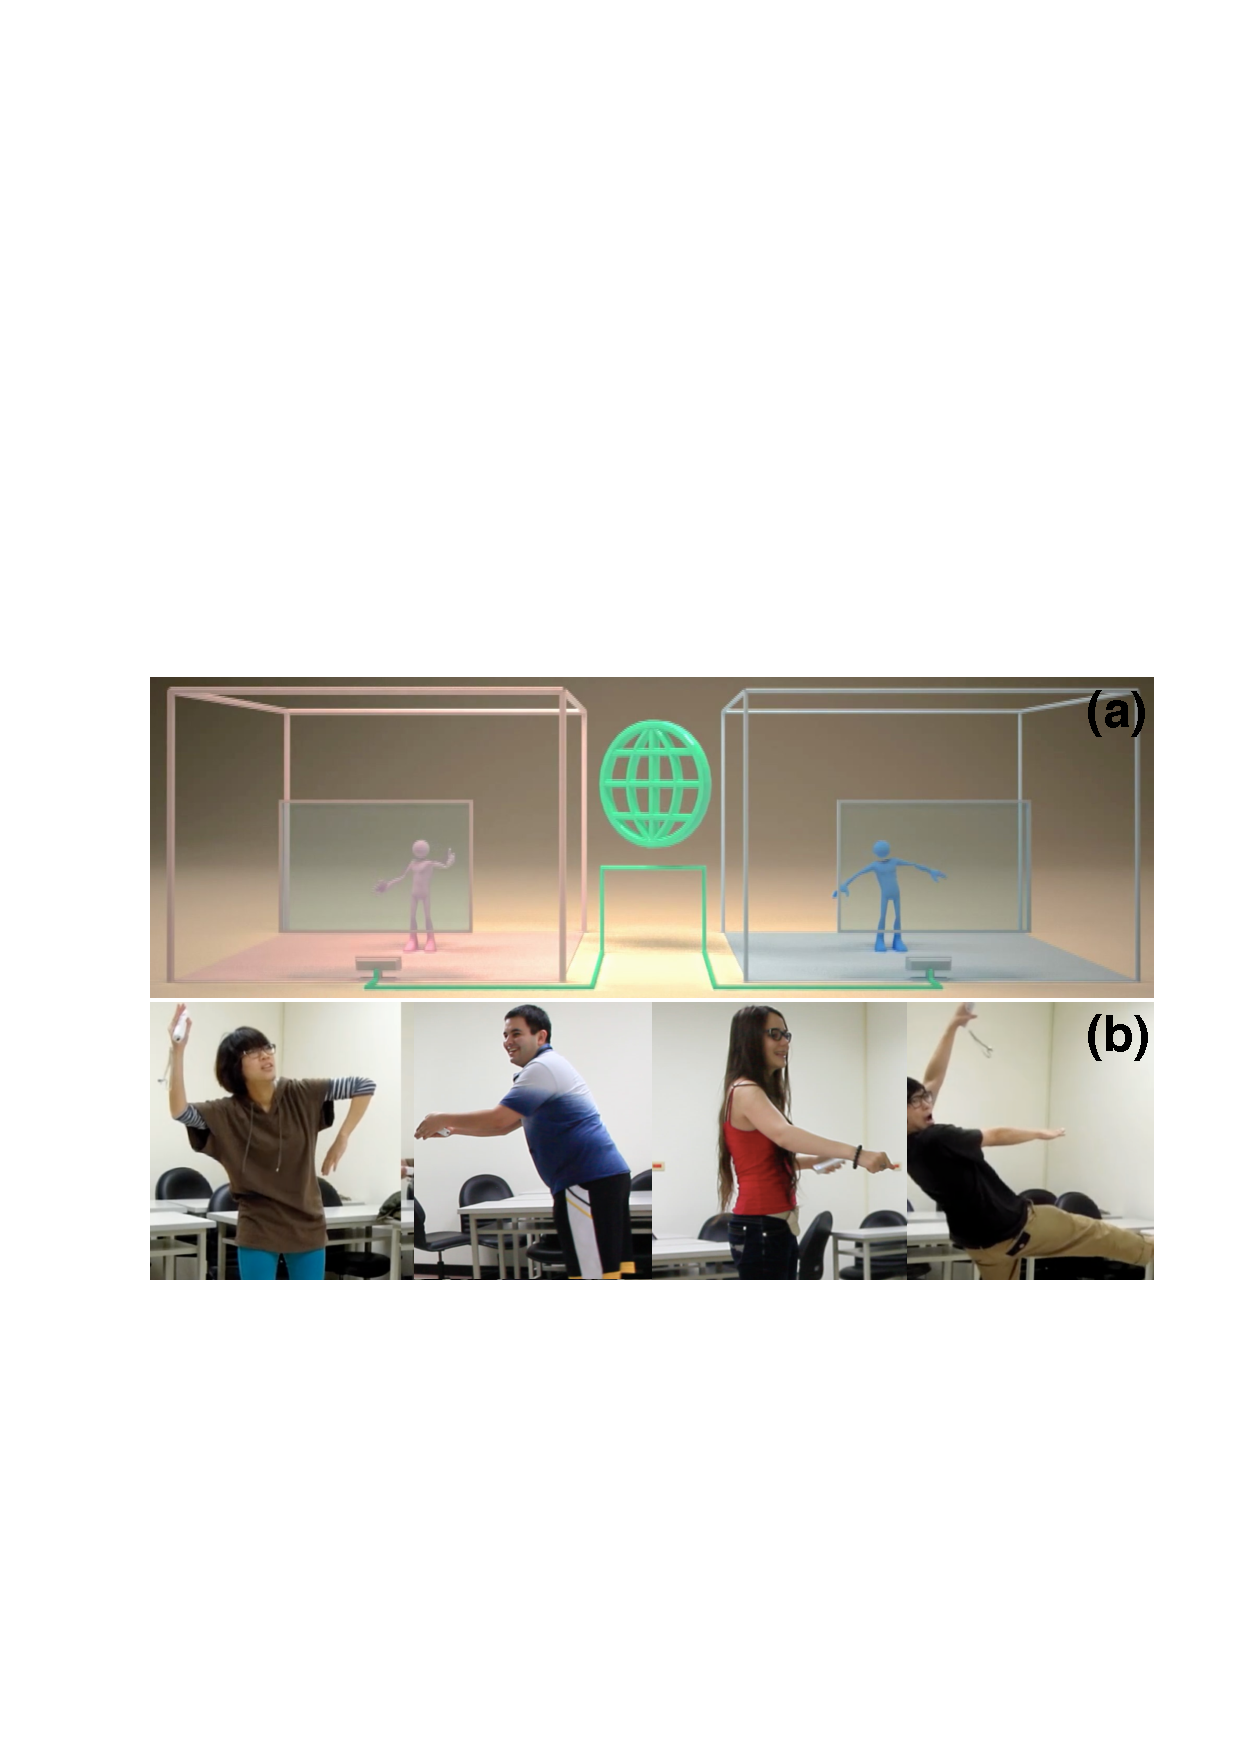
\includegraphics[width=0.9\columnwidth]{Figures/Topic.pdf}
\caption{(a) Playing cooperative games with body language over the Internet, (b) Body language expression from actual BodySense gameplay.}
\label{fig:Topic}
\end{figure}

We also developed a game using the BodyUp platform, called Mute Robot, that supports cooperative gaming in three communication modes: 1) speaking only, 2) body language only, and 3) both speaking and body language. We designed Mute Robot to enable pairs of players to cooperate to solve puzzles. It consists of three asymmetric puzzle stages, where only one player can see the solution hints and needs to guide the other player to solve the puzzles. Figure 1b) shows examples of body language expression during actual gameplay.

We conducted a 48-person user study using these three communication modes, with half of the users having common languages and half without.
% and  extended Short Feedback Questionnaire (eSFQ)\cite{eSFQ} and Cooperative Performance Metrics (CPMs)\cite{CPMs} to evaluate their gaming experience, the 
The study results showed that adding body language to cooperative games increased the fun and enjoyment ratings for all players (both with and without common languages) from an average of 3.8 to 4.4 (on a scale of 1 to 5). 

Also, in speaking-only mode, the negative co-experience reported by players without common languages was more than 3 times than that reported by players with common languages. Adding body language improved their positive co-experience by 33\% and reduced their negative co-experience by 73\%. 

In terms of preference, 75\% of the players with common language and 83\% of the players without common languages preferred having body language communication. Overall, 83\% of the players found having body language to be more cooperative.

% According to our final questionnaire, only 17\% and 25\% (different language group and common language group) player choose traditional communication manner (speaking) as the favorite manner.
%According to our final questionnaire, after adding the communication manner of body language, 83\% and 75\% (different language group and common language group) players choose our new communication manner (``body language'' and ``both'') as the favorite manner. 

%We also observe some interesting communication patterns. Game developer can make a better game experience with these information. We hope to inspire more exploration of using body language in game designs and spread game entertainment for more people.



